
\begin{defi}
    Uno \textbf{stimatore} è un oggetto che produce stime di $\vv{\theta}$
\end{defi}

Il nostro compito sarà quello di:\\
• Costruire gli stimatori\\
• Definire metodi per valutare gli stimatori\\

\begin{defi}
    Uno stimatore puntuale per $\theta$ è una qualunque funzione $W(X_1,...,X_n)$  del campione
\end{defi}

Oss. Ovvero uno stimatore è una statistica che usiamo per stimare $\theta$\\

Oss. Stimatore $\neq$ stima puntuale, che è la "realizzazione" dello stimatore: \ w$\, =W(\vv{X}(\omega))=W(x_1,...,x_n)$ \\

\subsection{Metodi per trovare stimatori}

\subsubsection{Metodo dei momenti} 

Partiamo dal campione $X_1,...,X_n$ iid $\Lc(X_i)$ funzione di $\vv{\theta}$\\
Momenti teorici: $\E{X}=\mu_1 \ \ \ \ \E{X^2}=\mu_2 \ \ \ \ \E{X^k}=\mu_k$ (quando esistono finiti)\\
Momenti campionari: $\frac{1}{n}\sum X_i= m_1 \ \ \ \ \frac{1}{n}\sum X_i^2 =m_2 \ \ \ \ \frac{1}{n}\sum X_i^k=m_k$\\

Oss. Di solito $\mu_j$ sono funzione di $\vt$\\



Lo stimatore sarà quella statistica che ottengo uguagliando $\mu_j=m_j$ anche se $\mu_j$ sono valori e $m_j$ sono VA\\

Def. $\widehat{F}_n(t)=\frac{1}{n}\Sum{i=1}{n}\II_{[X_i\le t]}$ detta \textbf{funzione di ripartizione empirica}, so che $\widehat{F}_n(t) \to F_X(t)$\\
Oss. I momenti di $F$ sono $\mu_j$, mentre i momenti di $\widehat{F}_n(t)$ sono gli $m_j$\\
Teorema: (Di Glivenko-Cantelli) \ \ \
Come $\widehat{F}_n(t)$ stima $F$, allora $m_j$ stimano i $\mu_j$\\

Risolvendo in $\theta_j$ il sistema: \ $ \begin{cases}
    m_1=\mu_1(\vt)\\
    \vdots \\
    m_h=\mu_h(\vt)
\end{cases}$ \ \ \ trovo gli stimatori $\hat{\theta}_{j, MOM}$ \\ \\


Esempio: $X_1,...,X_n \sim \Ec(\lambda)$\\
\[\mu_1=\E{X}=\frac{1}{\lambda}=m_1=\overline{X}_n \implies\hat{\lambda}_{MOM}=\frac{1}{\overline{X}_n}=\frac{n}{\sum X_i}\]

Esempio: $X_1,...,X_n \sim \Nc(\mu,\sigma^2)$ \ \ qui ho due incognite quindi dovrò usare almeno i primi due momenti\\
\[\begin{cases}
    \mu_1=\mu=\overline{X}_n\\
    \mu_2=\E{X^2}=\var{X}+\E{X}^2 = \theta_2+\theta_1^2 = m_2 = \frac{1}{n}\sum X_i^2
\end{cases}\]
\[ \text{Ottengo: \ }\begin{cases}
\hat{\mu}_{MOM}=\overline{X}_n\\
\hat{\sigma}^2_{MOM}=\frac{1}{n}\sum X^2_i -\overline{X}_n^2
\end{cases} \implies \begin{cases}
    \hat{\mu}=\overline{X}_n\\
    \hat{\sigma}^2_{MOM}=\frac{1}{n}\sum(X_i-\overline{X}_n)^2
\end{cases}\] \\

Esempio: $\camp \sim \Uc_{[-\theta,\theta]}$
\[\begin{cases}
    \mu_1=0\\
    \mu_2=\frac{4}{12}\theta^2=\frac{\theta^2}{3}
\end{cases} \ \implies \frac{\theta^2}{3}=\frac{1}{n}\sum X_i^2 \ \implies \hat{\theta}_{MOM}=\sqrt{\frac{3}{n}\sum X_i^2}\] \\

Valutiamo il metodo dei momenti\\
Pro: Sono equazioni algebriche, semplici da risolvere \\
Contro: Può succedere che le stime fornite da $\hat{\theta}_{MOM}$ non siano ammissibili, ovvero $\Hat{\theta}_{MOM}\not\in\Theta$\\ (esempio varianze negative)\\

Esempio: $\camp \sim Bi(k,p) \ \ \ \Theta = \NN \times [0,1]$
\[\begin{cases}
    \mu_1=kp=\overline{X}_n\\
    \mu_2=kp(1-p) + (kp)^2 = \frac{1}{n}\sum X_i^2
\end{cases} \ \implies  \begin{cases}
    \hat{p}=\frac{\overline{X}_n}{\hat{k}}\\
    \overline{X}_n - \hat{k}\frac{\overline{X}^2_n}{\hat{k}^2} + \hat{k}^2\O\frac{\overline{X}_n}{\hat{k}}\C^2 = \frac{1}{n}\Sum{i=1}{n}X_i^2 \end{cases}  \]\[ \implies \begin{cases}
        \hat{p}= \frac{\overline{X}_n}{\hat{k}}\\
        \overline{X}_n+\overline{X}_n^2 -\frac{1}{n}\sum X_i^2 = \frac{\overline{X}_n^2}{\hat{k}}
    \end{cases} \ \implies \begin{cases}
        \hat{p}= \frac{\overline{X}_n}{\Hat{k}}\\
        \hat{k}=\frac{\overline{X}_n^2}{\overline{X}_n-\frac{1}{n}\sum (X_i-\overline{X}_n)^2}
    \end{cases}\]\\   
Oss. É evidente che $\hat{k}$ non appartenga ai naturali\\



\Lezione{01/03/2023}


\subsubsection{Metodo basato sulla verosimiglianza}

\begin{defi}
$L(\vv{\theta},\vv{x})=f(\vv{x},\vv{\theta})$ \textbf{Likelihood} è la densità di $\vv{X}$ vista come funzione di $\vv{\theta}$
\end{defi}

Oss. Cercheremo il $\theta$ che massimizza la L, ovvero lo scenario più probabile\\

Esempio: Estrazione con reimmissione di 3 palline da un'urna che contiene una proporzione p incognita di palline bianche e (1-p) di palline nere\\
Sapendo di aver estratto due palline bianche su 3, scegliere tra $p=\frac{1}{2}$ e $p=\frac{1}{3}$\\

Dovrò calcolare la probabilità di aver estratto 2b su 3, sapendo il valore di p e valutare la probabilità più alta

\[\camp\sim Be(p) \ \ \sum X_i =2 \ \ \Lc(\Sum{i=1}{3}X_i)\sim Bi(3,p)\]
\[\PP_{p=\tfrac{1}{2}}(\sum X_i=2)=\binom{3}{2}\O\frac{1}{2} \C^2 \frac{1}{2}=\frac{3}{8} \ \ \ \PP_{p=\tfrac{1}{3}}(\sum X_i=2)=\binom{3}{2}\O\frac{1}{3} \C^2 \frac{2}{3}=\frac{2}{9}  \]
Osservo che $\frac{3}{8}>\frac{2}{9} \implies$ scelgo $p=\frac{1}{2}$\\

Oss. Ovviamente nel pratico non potremo tutte le volte calcolare la probabilità per ogni valore del parametro, ci servirà un metodo migliore\\

\begin{defi}
    \textbf{Stimatore di massima verosimiglianza} MLE (maximum likelihood estimator) $\hat{\theta}_{MLE}$ è il valore del parametro per cui $L(\theta,\vv{x})$ raggiunge il massimo \ \ \ $\hat{\theta}_{MLE}(\vv{x})=\underset{\theta \in \Theta}{ArgSup}\, L(\theta,\vv{x})$
\end{defi}

Valutiamo il metodo:\\
Pro: Per definizione le stime fornite da $\hat{\theta}_{MLE}$ sono sempre ammissibili, dato che prendo solo i valori $\theta\in\Theta$\\
Contro: Niente garantisce che ci sia un Max assoluto o che sia unico\\
Niente garantisce che il massimo si possa scrivere in forma chiusa, ovvero scriverlo in forma esplicita e quindi dovrò ricorrere a metodi di massimizzazione numerica\\

Quando possibile, il metodo per trovare il massimo sarà:\\
$\begin{cases}
    \frac{\partial L}{\partial \theta_i}=0 \ \ \forall i=1...k
\end{cases}$ \ \ \ Risolvendo questo sistema si ottiene l'equazione di verosimiglianza\\

Spesso, per esempio quando ho un campione, poiché le variabili sono indipendenti, avrò: \[L(\vv{\theta},\vv{x})=f(\vv{x},\vv{\theta})=\Prod{i=1}{n}f(x_i,\vv{\theta})\]
Però dato che il logaritmo è monotona crescente, vale $\underset{\theta \in \Theta}{ArgSup}(log\, L) = \underset{\theta \in \Theta}{ArgSup} (L)$\\
Definisco il logLiklihood $l(\vv{\theta},\vv{x})=log\, L(\vv{\theta},\vv{x})$ e risolvo $\begin{cases}
    \frac{\partial l}{\partial\theta_i}=0 \ \ \forall i=1...k
\end{cases}$\\
Inoltre è vantaggioso anche perché la derivata di un prodotto è brutta e la derivata della somma è bella\\ \\



Esempio: $\camp\sim Be(p)$
\[L(p,\vv{x})=\Prod{i=1}{n} p^{x_i}(1-p)^{1-x} \II_{\{0,1\}}(x_i) = p^{\sum x_i}(1-p)^{n-\sum x_i} \Prod{i=1}{n} \II_{\{0,1\}}(x_i) \]
\[  \textstyle l(p,\vv{x})=\sum x_i \ log(p) + (n-\sum x_i) log(1-p) + c(\vv{x}) \ \ \ \text{ posso non considerare tutto ciò che non dipende da p} \]
\[ \frac{\partial l}{\partial p} = \frac{\sum X_i}{p} - \frac{(n-\sum X_i)}{1-p} = 0\skipp\]
\[ (1) \ \ 0<\sum X_i < n \ \ \ \frac{\sum X_i}{p}=\frac{(n-\sum X_i)}{1-p} \Leftrightarrow \sum X_i -p\sum X_i = np - p\sum X_i \Leftrightarrow p=\frac{\sum X_i}{n} \implies \hat{p}_{MLE}=\overline{X}_n\]
$ \displaystyle (2) \ \sum X_i =0 \ \ \ \frac{\partial l}{\partial p}= -\frac{n}{1-p}<0 \implies \hat{p}_{MLE}=0=\overline{X}_n $\skipp\\
$\displaystyle(3) \  \sum X_i = n \ \ \ \frac{\partial l }{\partial p}=\frac{n}{p}>0 \implies \hat{p}_{MLE}=1=\overline{X}_n $
\[\text{Quindi: } \ \hat{p}_{MLE}=\overline{X}_n\] \\

Esempio: $\camp \sim \Uc_{[0,\theta]}$
\[L(\theta,\vv{x})=\frac{1}{\theta^n}\Prod{i=1}{n} \II_{[0,\theta]}(x_i)=\frac{1}{\theta^n}\II_{[0,\theta]}(X_{(n)})\]
\[\II_{[0,\theta]}(X_{(n)}) \Leftrightarrow 0\le X_{(n)}\le \theta \Leftrightarrow \II_{[X_{(n)},+\infty]}(\theta) \implies \ L\O\theta,\vv{x}\C=\frac{1}{\theta^n}\II_{[X_{(n)},+\infty]}(\theta)\]
\begin{wrapfigure}{r}{0.25\textwidth}
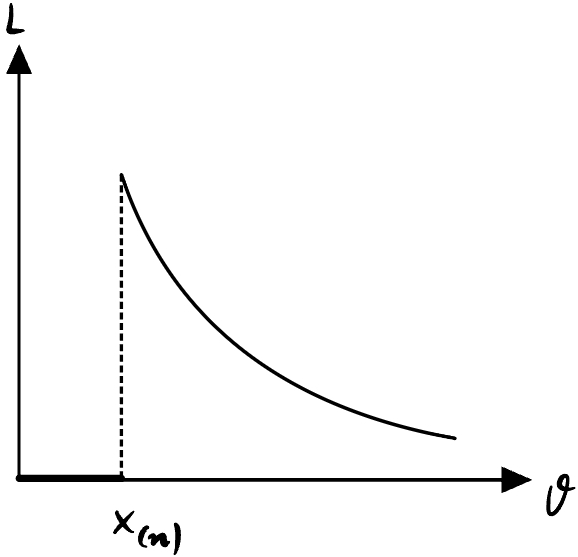
\includegraphics[width=0.17\textwidth]{Figura1.jpeg}
\end{wrapfigure}
\phantom{x}

In questo caso non serve fare calcoli, basta fare il disegno\\
Notiamo subito che il massimo della funzione L è in $X_{(n)}$\\
$ \implies \hat{\theta}_{MLE}=X_{(n)}$\\ \\

Confrontiamo questo caso tra i due metodi visti:
$\mu_1=\frac{\theta}{2}\implies \hat{\theta}_{MOM}=2\overline{X}_n$, mentre \ \ $\hat{\theta_{MLE}}=X_{(n)}$\\
In questo caso useremo $X_{(n)}$ perché è una statistica sufficiente, minimale e completa, quindi più comoda\\ \\


Esempio: $\camp\sim\Nc (\mu,\sigma^2)$
\[k=2 \ \ \ L(\mu,\sigma^2,\vv{x})=\frac{1}{(2\sqrt{2\pi\sigma^2})^2}  \, exp \OOO -\frac{1}{2\sigma^2}\Sum{i=1}{n} (x_i-\mu)^2 \CCC  \implies l(\mu,\sigma^2,\vv{x})=-\frac{n}{2} log (2\pi\sigma^2) - \frac{1}{2\sigma^2}\Sum{i=1}{n}(x_i-\mu)\]
Cerco i punti in cui la derivata di L cambia di segno e poi verifico se sono effettivamente massimi di L
\[ \begin{cases}
    \frac{\partial l}{\partial \mu}=\frac{1}{\sigma^2}\sum (X_i-\mu)\\
    \frac{\partial l}{\partial \sigma^2} = -\frac{n}{2}\frac{2\pi}{2\pi\sigma^2}+\frac{\sum (X_i-\mu)^2}{2(\sigma^2)^2}
\end{cases} \ \ \ \begin{cases}
    \frac{\partial l}{\partial \mu}\ge 0 \Leftrightarrow \sum X_i \ge n\mu \Leftrightarrow \mu \le \frac{\sum X_i}{n}\\
    \frac{\partial l}{\partial \sigma^2}\ge 0 \Leftrightarrow \frac{\sum (X_i-\mu)^2}{\sigma^2} \ge n \Leftrightarrow \sigma^2\le \frac{\sum (X_i-\mu)^2}{n}
\end{cases} \]   \[\text{ Nella 2° equazione ho il parametro $\mu$, lo devo sostituire con il suo stimatore: } \ \ \begin{cases}
    \hat{\mu}_{MLE}=\overline{X}_n\\
    \hat{\sigma^2}_{MLE}=\frac{\sum(X_i-\overline{X}_n)^2}{n}
\end{cases}\] \\



Proprietà di \textbf{invarianza} degli MLE dice che se $\hat{\theta}_{MLE}$ è lo stimatore MLE di $\theta \implies \ \forall \tau$ funzione di $\theta$,\\ lo stimatore MLE di $\tau(\theta)$ è $\tau(\hat{\theta}_{MLE})$, ovvero $\hat{\tau(\theta)}_{MLE}=\tau(\hat{\theta}_{MLE})$\\ \\

Esempio: $\camp\sim \Pc(\lambda)$ \ \ trovare l'MLE di $\prob{X_i=0}= e^{-\lambda}$\\
Userò la proprietà di invarianza, cerco $\hat{\lambda}_{MLE}$
\[L(\lambda,\vv{x})=\Prod{i=1}{n} \frac{e^{-\lambda}\lambda^{x_i}}{x!}\II_{\NN}(x_i)\]
\[\frac{\partial l}{\partial \lambda}=\Sum{i=1}{n} \frac{\partial}{\partial \lambda} \O log \O\frac{e^{-\lambda}\lambda^{X_i}}{X!}\C\C = \Sum{i=1}{n}\frac{\partial}{\partial \lambda} (-\lambda + X_i log\lambda) = \sum (-1 +\frac{X_i}{\lambda} = -n + \frac{\sum X_i}{\lambda})   \] 
\[ \frac{\partial l}{\partial \lambda}\ge 0 \Leftrightarrow \lambda\le \frac{\sum X_i}{n} \implies \hat{\lambda}_{MLE}=\overline{X}_n \]
\[ \implies \hat{(e^{-\lambda})}= e^{-\overline{X}_n} \text{per principio invarianza}\] \\

Esempio: Abbiamo appena calcolato lo stimatore $\hat{\sigma^2}_{MLE}$ per un campione gaussiano, allora vale:
\[\hat{\sigma}_{MLE}=\sqrt{\hat{\sigma^2}_{MLE}}=\sqrt{\frac{\Sum{i=1}{n}(X_i-\overline{X}_n)^2}{n}}\]

Esempio: Sapppiamo che $\hat{p}_{MLE}=\overline{X}_n$, allora
\[\sigma^2=\tau(p)=p(1-p)\implies \hat{\sigma^2}_{MLE}=\overline{X}_n(1-\overline{X}_n)\] \\




Restrizione del Range:\\
Se restringo lo spazio dei parametri da $\theta\in\Theta$ a $\theta \in \Theta_0 \subset \Theta$, \ allora \ \ $\hat{\theta^0_M}_{LE} = \underset{\theta\in\Theta_0}{ArgSup} L(\theta,\vv{x})$\\



\Lezione{03/03/2022}

\subsection{Analisi degli stimatori}

\begin{defi}
    Il MSE (mean squared error) è l'errore quadratico medio di uno stimatore $T$ per un parametro incognito $\theta$ ed è definito nel seguente modo: \ \ $MSE_{\theta}(T)=\EE_{\theta}[(T-\theta)^2]$
\end{defi}

\[MSE_{\theta}(T)=\EE_{\theta}[(T-\EE_{\theta}[T]+\EE_{\theta}[T]-\theta)^2]=\EE_{\theta}[(T-\EE_{\theta}[T])^2+(\EE_{\theta}[T]-\theta)^2+2(T-\EE_{\theta}[T])(\EE_{\theta}[T]-\theta)] = \]\[ =\EE_{\theta}[(T-\EE_{\theta}[T])^2] + (\EE_{\theta}[T]-\theta)^2 + 0\ \ \implies MSE_{\theta}(T)=Var_\theta[T]+(\EE_{\theta}[T]-\theta)^2\]\\
%
Definiamo la distorsione = bias := $\EE_{\theta}[T]-\theta $ \\
Se $\EE_{\theta}[T]-\theta =0$, allora T è detto non distorto per $\theta$ o unbiased\\

Oss. Tendenzialmente esiste un trade-off tra varianza e distorsione, per cui è difficile tenerli bassi entrambi\\

Dato $\camp $ \ la media campionaria $ \overline{X}_n$ è sempre uno stimatore non distorto della $\E{X_i}$\\
Infatti
$\E{\overline{X}_n}=\E{\frac{1}{n}\sum X_i}=\frac{1}{n}n\E{X}=\E{X}$\\

Dato $\camp\sim\Nc(\mu,\sigma^2)$ confrontiamo due stimatori della varianza\\
$S^2=\frac{1}{n-1}\Sum{i=1}{n}(X_i-\overline{X}_n)^2 \hspace{30pt} \hat{\sigma}^2_{MLE} = \frac{1}{n}\Sum{i=1}{n}(X_i-\overline{X}_n)^2=S_0^2$ \\
Oss. Possiamo sfruttare il fatto che $\frac{(n-1)S^2}{\sigma^2}\sim\Chi^2(n-1)\sim\Gamma\O\frac{n-1}{2},\frac{1}{2}\C$

\[MSE(S^2)=\var{S^2}+(\E{S^2}-\sigma^2)^2 =\OOO\OOO \E{S^2}=\frac{\sigma^2}{n-1}\E{\Chi^2(n-1)}=\sigma^2  \CCC\CCC= \var{S^2}= \]\[= \frac{\sigma^4}{(n-1)^2}\var{\Chi^2(n-1)}=\frac{\sigma^4}{(n-1)^2}(n-1)2=\frac{2\sigma^4}{n-1}\]
\[S_0^2=\frac{n-1}{n}S^2 \implies \ \text{Bias}=\E{S_0^2}-\sigma^2=\frac{n-1}{n}\sigma^2-\sigma^2=-\frac{\sigma^2}{n} \ \ \ \O S_0^2 \text{ sottostima }\sigma^2\C\]
\[ \implies \var{S_0^2}=\frac{(n-1)^2}{n^2}\var{S^2}=\frac{2\sigma^4(n-1)}{n^2}\]

\[MSE(S_0^2)=\frac{2\sigma^4(n-1)}{n^2}+\frac{\sigma^4}{n^2} = \frac{(2n+1)\sigma^4}{n^2}\]

\[\text{Confrontiamo i due MSE: } \hspace{30pt} \frac{2\sigma^4}{n-1} \hspace{30pt} \frac{(2n+1)\sigma^4}{n^2} \]
\[\text{Equivale al confronto tra: } \ \ \ \ \forall\sigma^2 \ \ \ \ (2n-1)(n-1)= 2n^2 -3n +1  \ \ \ \ \text{ e } \ \ \ \ 2n^2\]
\[\text{E quindi: } \ \ \ \ 1-3n \ \ \ \text{ e } \ \ \ 0  \ \ \ \
\ \ 
\text{ Dove il primo è sempre miore del secondo}\]\\
%
Qunidi $\forall \sigma^2 \ \ \ MSE_{\sigma^2}[S_0^2]<MSE_{\sigma^2}[S^2]$ \ \ ovvero mi conviene prendere uno stimatore distorto\\
Questo perchè la varianza è sempre inversa all'errore, quindi conviene sovrastimare l'errore per essere cauti\\

Definiamo le seguenti relazioni tra stimatori e parametri:\\
Se $\E{T}<\theta$ sottostima\\
Se $\E{T}>\theta$ sovrastima\\



In generale tra due stimatori $T_1$ e $T_2$ di $\theta$, scelgo lo stimatore con MSE inferiore\\
$T_1$ è preferibile a $T_2$ se $MSE_{\theta}(T_1)<MSE_{\theta}(T_2) \ \ \forall \theta$\\

Attenzione che il confronto tra MSE è un confronto tra due funzioni di $\theta$, potrebbe succedere che la disuguaglianza tra MSE non sia vera $\ \forall\theta$ \\
Ovvero che l'ordinamento del confronto tra MSE non è totale, potrebbero esserci stimatori non confrontabili\\ \\






Esempio: $\camp$ con $\Lc(x,\theta)$ che hanno $\theta=\E{X_i}$ e $1=\var{X_i}$\\
$T_1=\overline{X}_n \ \ T_2=a\overline{X_n}$\\
\[MSE_{\theta}[T_1]=Var_{\theta}[T_1]=\var{\frac{1}{n}\sum X_i}=\frac{1}{n^2}\cdot n\cdot 1=\frac{1}{n}\]
\[MSE_{\theta} [T_2] = \frac{a^2}{n}+(a\theta-\theta)^2=\frac{a^2}{n}+(a-1)^2\theta^2\]

% fatta la Figura1c in testo, ma brutta

\fg[]{0.3}{Figura1b.jpeg}

I due stimatori sono non confrontabili, però sceglierò la media campionaria, perché l'errore rimane "sotto controllo", mentre l'altro errore è quadratico\\ \\



Esempio: $X_1\sim \Pc(\lambda) \ \ \ T(X_1)=(-1)^{X_1}$ 
\[\E{T}= \E{(-1)^{X_1}}=\Sum{k=0}{+\infty}\OO(-1)^k\frac{e^{-\lambda}\lambda^k}{k!}\CC = e^{\lambda} \OO\Sum{k=0}{+\infty}\frac{(-\lambda)^k}{k!}\CC=e^{-2\lambda}\]
T è uno stimatore non distorto di $e^{-2\lambda}$ \ \ \  \ \ $T=\begin{cases}
    1 \ \ \text{ se $X_1$ è pari}\\
    -1 \ \ \text{ se $X_1$ è dispari}
\end{cases}$ \\

Oss. Sto però stimando con -1 la funzione $e^{-2\lambda}$  che è sempre positivo e non potrà mai essere -1, inoltre posso ricavare che il MSE non è tanto basso\\
Oss. Questo controesempio mi dice che non è detto che uno stimatore unbiased sia buono.
Proviamo a restringere il campo degli stimatori che cerchiamo\\


\begin{defi}
    Per UMVUE si intente uniform minimum variance unbiased estimator, ovvero stimatore non distorto a varianza uniformemente minima (rispetto a $\theta$)\\
    $T^*$ è \textbf{UMVUE} per $\theta$ se \ $\begin{cases}
        \EE_{\theta}[T^*]=\theta\\
         \E{T}=\theta \implies \var{T^*}\le\var{T}\  \ \ \  \forall \theta \ \ \  \forall T \text{ stimatore non distorto di } \theta
    \end{cases}$
\end{defi}
\phantom{}\\

\begin{teo}[Disuguaglianza di Cramer-Rao]
Siano $\camp \ iid $ con $ X_i\sim f(x_i,\theta) $ e $ T(\camp)$ stimatore di $\theta$. Assumiamo che:\\
i)\ supporto di $X_i$ non dipende da $\theta$ \ \ \ \ ii)\ $\E{T^2}<+\infty$ \smallskip \\
iii) \ $\frac{d \EE_{\theta}[T]}{d\theta}=\frac{d}{d\theta}\displaystyle\int_{\R^n} T(\vv{x})f(\vv{x},\theta)\,d\vv{x}=\int_{\R}T(\vv{x})\frac{\partial}{\partial \theta}f(\vv{x},\theta)\,d\vv{x}$
\[ \text{Allora} \ \ \ \ \ \ 0<\EE_{\theta}\OO\O\frac{\partial}{\partial\theta}\,log \,f(\vv{X},\theta)\C^2\CC<+\infty \ \implies \var{T}\ge\frac{\OO\frac{d}{d\theta}\EE_{\theta}[T]\CC^2}{\EE_{\theta}\OO\O\frac{\partial}{\partial\theta}\,log\,f(\vv{X},\theta)\C^2\CC}\]
\end{teo}

%
Oss. Nella famiglia esponenziale le condizioni sono rispettate\\
Oss. Inoltre se siamo nei non distorti, allora  $\frac{d}{d\theta}\EE_{\theta}[T] =1$\\

Informazione di Fisher = $I_n(\theta)=\EE_{\theta}\OO\O\frac{\partial}{\partial\theta}\,log\,f(\vv{X},\theta)\C^2\CC$\\
Oss. Detta informazione perché se ho I bassa significa che il limite sopra cui deve stare la varianza degli stimatori è alta e viceversa e quindi mi dice in anticipo che tipo di stimatori potrò trovare \\ \\

Nella classe degli stimatori non distorti il limite di C.-R. è $\frac{1}{I_n(\theta)} \ \implies \var{T}\ge\frac{1}{I_n(\theta)}$\\

Se io trovo uno stimatore T non distorto la cui varianza raggiunge il limite di C.-R. allora T è UMVUE\\
Però l'UMVUE può non raggiungere necessariamente il limite di C.-R.\\ \\


\Lezione{07/03/2023}


Esempio: Trovaiamo l'informazione di Fisher per delle Poisson \ \ \ $\camp\sim\Pc(\lambda)$ \[I_n(\lambda)=\E{\O\frac{\partial}{\partial \lambda}\,log\,f(\vv{X},\lambda)\C^2}
\]
\[\frac{\partial}{\partial\lambda}\,log\,f(\vv{X},\lambda)=\frac{\partial}{\partial\lambda}\,log\OO\Prod{i=1}{n}\frac{e^{-\lambda}\lambda^{X_i}}{X!}\CC=\Sum{i=1}{n}\frac{\partial}{\partial\lambda}\,log\,(e^{-\lambda}\lambda^{X_i})=\Sum{i=1}{n}\frac{\partial}{\partial\lambda}(-\lambda+X_i\,log\,\lambda)=\Sum{i=1}{n}\O-1+\frac{X_i}{\lambda}\C=\frac{n}{\lambda}\O\overline{X}_n-\lambda\C\]
\[\implies I_n(\lambda)=\E{\O\frac{n}{\lambda}(\overline{X}_n-\lambda)\C^2}=\frac{n^2}{\lambda^2}\E{\O\overline{X}_n-\lambda\C^2} = \frac{n^2}{\lambda^2}\var{\overline{X}_n}=\frac{n^2}{\lambda^2}\cdot\frac{\lambda}{n}=\frac{n}{\lambda} \skipp\skipp\]


Oss. Spesso aiuta, nel calcolo di I, riportarsi a una varianza nota, come abbiamo fatto qui\\

Abbiamo quindi ottenuto che $\var{T}\ge\frac{\OO\frac{d}{dx}\E{T}\CC^2}{I_n(\lambda)}=\frac{\lambda}{n}$ dato che lo stimatore è non distorto\\

Osservo che $\overline{X}_n$ è non distorto e $\var{\overline{X}_n}=\frac{\lambda}{n}$ \ cioè raggiunge il limite di C.-R. \ $\implies \overline{X}_n$ è UMVUE per $\lambda$\\

\begin{Dim}[Cramer-Rao]
La dimostrazione di C.-R. è un'applicazione della disuguaglianza di Cauchy-Schwarz:
\[ |\cov{X}{Y}|^2 \le \var{X}\var{Y} \skipp\]
%
Per dimostrare C.-S. \ considero una va \ $aX+Y$
\[
0\le\var{aX+Y}=\underset{\text{Polinomio di ordine 2 in a}}{\underbrace{a^2\var{X}+2a\cov{X}{Y}+\var{Y}}}\]
Ho quindi ottenuto una parabola che so essere sempre positiva e quindi ha determinate non positivo 
\[\Delta=4\cov{X}{Y}^2 -4\var{X}\var{Y}\le 0\]
\[\implies \var{X}\ge\frac{|\cov{X}{Y}|^2}{\var{Y}} \]
\phantom{}

Si useranno come variabili \ $X=T \ \text{ e } \ Y=\frac{\partial}{\partial\theta}\,log\,f(\vv{X},\theta)$\\

Per l'ipotesi iii) del teorema vale: \ \  \ $ \frac{d}{d\theta}\EE_{\theta}[T] = \displaystyle\int_{\R^n}T(\vv{x})\frac{\partial}{\partial \theta}f(\vv{x},\theta)\,d\vv{x} $
\[
\frac{\partial}{\partial\theta}\EE_{\theta}[T]\overset{(3)}{=} \int_{\R^n}T(\vv{x})\cdot\frac{\partial}{\partial\theta}f(\vv{x},\theta)\,d\vv{x} = \int_{\R^n}T(\vv{x})\cdot\frac{\partial}{\partial\theta}\,log\,f(\vv{x},\theta)\cdot f(\vv{x},\theta)\, d\vv{x} = \E{T\cdot Y}\]
\phantom{}

\[\text{Posto \ } T(\vv{X})=1 \ \text{ allora \ } \ 0=\frac{d}{d\theta}\E{1}=\int_{\R^n}\frac{\partial}{\partial\theta}\,f(\vv{x},\theta)\,d\vv{x}=\int_{\R^n}\frac{\partial}{\partial\theta}\,log\,f(\vv{x},\theta)\cdot f(\vv{x},\theta)\,d\vv{x} \]
\[\implies \ \E{Y}=0 \ \implies \ \cov{X}{Y}=\E{X\cdot Y} \ \text{ e } \ \var{Y}=\E{Y^2}\]\\

Adesso per ricavare C.-R. dobbiamo applicare C.-S.\\
\[\var{T}\ge\frac{\cov{T}{Y}^2}{\var{Y}}=\frac{\O\frac{d}{d\theta}\EE_{\theta}[T]\C^2}{\E{Y^2}}=\frac{\OO\frac{d}{d\theta}\EE_{\theta}[T]\CC^2}{\EE_{\theta}\OO\O\frac{\partial}{\partial\theta}\,log\,f(\vv{x}\theta)\C^2\CC}\]
\end{Dim}




Dalla dimostrazione si deduce che nella disuguaglianza C.-R. si raggiunge l'uguale quando \\ $X=T(\vv{x})$ è trasformazione lineare di $Y=\frac{\partial}{\partial\theta}\,log\,f(\vv{x},\theta)$




\subsubsection*{Ricerca dell'UMVUE}

\begin{teo}[Rao-Blackwell]
Siano T uno stimatore non distorto per $\theta$ e W una statistica sufficiente \\
Poniamo $M=\EE_{\theta}[T|W]$, \ allora M è ancora uno stimatore non distorto per $\theta$ e \ $\text{Var}_{\theta}[M]\le \text{Var}_{\theta}[T]$
\end{teo}

\begin{Dim}
1) M è uno stimatore
\[
M=\EE_{\theta}[T(\vv{X})|W]=\int_{\R^n} T(\vv{x})f(\vv{x}|W)\,d\vv{x} \] \[ \text{W è suff} \implies f(\vv{x}|W) \text{ non dipende da } \theta \implies \text{M stimatore}
\]
2) M è non distorto
\[
\EE_{\theta}[M]=\EE_{\theta}[\EE_{\theta}[T|W]]=\EE_{\theta}[T]=\theta
\]
3) $\var{M}\le\var{T}$
\[
\var{T}=\var{\EE_{\theta}[T|W]} + \underset{\ge0 \text{ perché var}\ge0}{\underbrace{\EE_{\theta}[\var{T|W}]}} \ \implies \var{M}\le\var{T}
\]
\end{Dim}

Vogliamo far vedere che con W non sufficiente, non vale il teorema

Esempio: $X_1,X_2\sim\Nc(\mu,1)$ \ \ \ $T=\frac{X_1+X_2}{2} \ \ \ \ W=X_1$
\[\E{T|W}=
\E{\overline{X}_2|X_1}=\frac12\OO\E{X_1|X_1}+\E{X_2|X_1}\CC= \frac12\O X_1+\mu\C \ \  \text{ Non è uno stimatore}
\]\\
%
\begin{teo}[Unicità dell'UMVUE]
    Sia $T(\vv{X})$ UMVUE per $\theta$, allora T è unico
\end{teo}

\begin{Dim}
    Supponiamo che esista un altro $T'$ UMVUE per $\theta$\\
    Ne costruisco un terzo. Sia $T^*=\frac12(T+T')$\\
    $T^*$ è uno stimatore e ha $\E{T^*}=\frac12(\E{T}+\E{T'})=\theta \ \implies$ \ anche $T^*$ è non distorto\\
    \[
    \var{T^*}=\frac14 \OO\var{T}+\var{T'}+2\cov{T}{T'}\CC \ \overset{C.-S.}{\le} \ \frac14\OO\var{T}+\var{T'}+2\sqrt{\var{T}\cdot\var{T'}}\CC
    \]
    Però dato che $T$ e $T'$ sono UMVUE allora devono avere stessa varianza
    $\implies \var{T^*}\le \var{T}$ Ma dato che T è UMVUE e $T^*$ è non distorto, in C.-S. vale l'uguaglianza $ \implies \var{T^*}=\var{T}$\\
    L'unico modo per cui questo è possibile è se $T'=aT+b$\\
    \[\var{T}=\cov{T}{T'}=\cov{T}{aT+b}=a\var{T} \implies a=1\]
    \[\E{T}=\E{T'}=\E{aT+b}=\E{T}+b \ \implies b=0\]
    \[\implies T=T' \implies \text{Se T esiste è unico}\]
\end{Dim}

\begin{teo}[Lemma di Scheffè 2]
    Sia T stimatore non distorto per $\theta$ (e quindi per ogni funzione $\tau(\theta)$)\\
    Sia W stat suff, minimale e completa per $\theta$\\
    Allora $M=\EE_{\theta}[T|W]$ è (l'unico) UMVUE per $\theta$
\end{teo}



\Lezione{13/03/20}


\begin{Dim}
    M è uno stimatore, dato che W è sufficiente (visto in Cramer-Rau)
    \[
    \EE_{\theta}[M]=\EE_{\theta}[\EE_{\theta}[T|W]]= \EE_{\theta}[T]=\theta
    \]
    Supponiamo che M non sia UMVUE, ovvero che esista uno stimatore T' non distorto di $\theta$ tc \ $\var{T'}<\var{T}$\\
    Usiamo teorema Rao-Blackwell su $T'$\\
    $M'=\E{T'|W}$ è uno stimatore non distorto di $\theta$ con $\var{M'}\le\var{T'}<\var{M}$\\

    Osserviamo che $M$ e $M'$ sono funzioni di $W$ e quindi $(M-M')$ è anch'essa funzione di $W$
    \[
    \E{M-M'}=0 \implies M-M' \text{ è una funzione } g(W) \text{ con media nulla, ma $W$ completo }\]
    \[\implies \prob{g(W)=0}=1 \implies M=M' \text{ qc}
    \]
    Ma questo contraddice l'affermazione che M non fosse UMVUE, quindi lo è ed è unico\\
\end{Dim}



Esempio: $\camp\sim Bi(k,\theta)$ con $k$ fissato e $\theta$ incognito

Cerchiamo l'UMVUE per $\tau(\theta)=\prob{X_i=1}=k\theta(\-\theta)^{k-1}$

Sappiamo che $W=\sum X_j$ è stat suff min completa per un campione binomiale, dove $W\sim Bi(nk,\theta)$

Però $\E{W}=nk\theta \ne \tau(\theta)$, quindi mi devo trovare uno stimatore che condizionato a $W$ mi dia $\tau$\\

Quando $\tau (\theta)$ è una probabilità, posso prendere delle bernulli che abbiano p uguale a $\tau$

\[
Y_1,...,Y_n \text{ tc } \   Y_i=\begin{cases}
    1 \ \ \ \text{ se } X_i=1\\
    0 \ \ \ \text{ se } X_i\ne 1
\end{cases} \ \ \implies \ \ Y_i\sim \II_{X_i=1} \sim Be (\prob{x_i=1}) = Be\O k\theta(1-\theta)^{k-1}\C
\]

Quindi $\overline{Y}_n =\frac1n \Sum{i=1}{n} Y_i$ è stimatore non distorto di $\tau(\theta)$\\

Adesso devo fare l'attesa condizionata, che è la parte più "contosa":
\[
\text{UMVUE per } \tau(\theta) \text{ è } \E{\overline{Y}_n \Big| \Sum{j=1}{n}X_j}  = \frac{1}{n} \Sum{j=1}{n} \E{Y_i \Big| \sum X_j } \ \overset{\text{sono iid}}{ = } \ \E{Y_1 \Big| \sum X_j }
\]
\[
\text{Però \ } \E{Y_1 \Big| \sum X_j = t } = \prob{Y_1=1 \Big| \Sum{j=1}{n} X_j =t } = \frac{\prob{Y_1=1 \cap \sum X_j =t}}{\prob{\sum X_j=t}} = \frac{\prob{X_1=1 \cap \sum X_j =t}}{\prob{\sum X_j=t}}= 
\]
Adesso gli eventi al numeratore non sono indipendenti, quindi non posso spezzare l'intersezione, però posso renderli indipendenti:
\[
=\frac{\prob{X_1=1 \cap \Sum{j=2}{n} X_j =t -1 }}{\prob{\sum X_j=t}} = \frac{\prob{X_1=1 } \prob{ \Sum{j=2}{n} X_j =t -1 }}{\prob{\sum X_j=t}}=
\]

Dove \ \ $X_j \sim Bi(k,\theta)$ \ \ $ \Sum{j=2}{n} X_j \sim Bi((n-1)k,\theta)  \ \ \Sum{j=1}{n} X_j \sim Bi(nk,\theta) $
\[
=\frac{k\theta (1-\theta)^{k-1} \binom{(n-1)k}{t-1} \theta^{t-1}(1-\theta)^{(n-1)k -t +1} }{\binom{nk}{t} \theta^t (1-\theta)^{nk-t}} = \frac{\binom{(n-1)k}{t-1} k }{\binom{nk}{t}  } = \E{Y_1 \big| \sum X_j =t}
\]

Quindi l'UMVUE per \  $k\theta(1-\theta)^{k-1}$ \  è \  \ $\displaystyle \frac{\binom{(n-1)k}{ \sum X_j -1 } k }{\binom{nk}{\sum X_j}  } = \E{\overline{Y}_n \big| \sum X_j } $\\



\subsection{Informazione di Fisher}

\begin{defi}
    Informazione di Fisher = $I_n(\theta)=\EE_{\theta}\OO\O\frac{\partial}{\partial\theta}\,log\,f(\vv{X},\theta)\C^2\CC$
\end{defi}

\textbf{Lemma1:}\\
Sia $\camp$ iid, allora $I_n(\theta)=nI_1(\theta)=n \E{\O\frac{\partial}{\partial\theta} \,log \,f(X_1,\theta)\C^2}$\\

\begin{Dim}[Lemma1]
    \[
    I_n(\theta)=\EE_{\theta}\OO\O\frac{\partial}{\partial\theta}\,log\, \Prod{i=1}{n} f(X_i, \theta)\C^2\CC = \EE_{\theta}\OO\O \Sum{i=1}{n} \frac{\partial}{\partial\theta}\,log\,  f(X_i, \theta)\C^2\CC  \]
    Quando lavoriamo con l'informazione di Fisher le ipotesi per la disuguaglianza di Cramer-Rao le ho sempre, quindi posso scambiare integrale e derivata e avevamo visto che grazie a questo vale:
    \[\E{ \frac{\partial }{\partial \theta} \, log\, f(X_i,\theta) }=0 \ \ \text{ quindi posso scrivere la media del quadrato con la varianza}\]
    \[
    I_n(\theta)= \var{\Sum{i=1}{n} \frac{\partial}{\partial\theta}\,log\,  f(X_i\theta)} \ \overset{ind}{ = } \  \Sum{i=1}{n}\var{ \frac{\partial}{\partial\theta}\,log\,  f(X_i,\theta)} \ \overset{iid}{ = } \ n \var{\frac{\partial}{\partial\theta}\,log\,  f(X_i,\theta)} =
    \]
    \[ \text{Per quanto detto prima } \ \ = n \E{ \O \frac{\partial}{\partial\theta}\,log\,  f(X_i,\theta)\C^2 } = n I_1(\theta) \]
\end{Dim}


\textbf{Lemma2:}\\
Se in aggiunta alle condizioni di Cramer-Rao si ha che: \ \ $ \frac{\partial }{\partial \theta} \OO \int_{\R^n} \frac{\partial }{\partial \theta} \, f(\vv{x}, \theta) \, d\vv{x}  \CC = \int_{\R^n} \frac{\partial^2}{\partial\theta^2}\, f(\vv{x},\theta)\, dx$\\
Allora $I_n(\theta) = - \EE_{\theta} \OO \frac{\partial^2}{\partial\theta^2}\, log \, f(\vv{x},\theta) \CC$\\




\begin{Dim}[Lemma2]
    \phantom{}\vspace*{-15pt}
    \[\E{\frac{\partial^2}{\partial\theta^2}\, log\, f(\vv{x},\theta)} = \int_{\R^n} \frac{\partial^2}{\partial\theta^2}\O log\, f(\vv{x},\theta)\C \cdot f(\vv{x},\theta)\, d\vv{x} = \int_{\R^n} \frac{\partial }{\partial \theta} \O \frac{ \frac{\partial }{\partial \theta} \, f(\vv{x},\theta)  }{f(\vv{x},\theta)}\C\, f(\vv{x},\theta) \, d\vv{x}=\] 
    \[= \int_{\R^n} \frac{\partial^2 }{\partial \theta^2} f(\vv{x},\theta)\cdot \frac{1}{f(\vv{x},\theta)} f(\vv{x},\theta)\, d\vv{x} + \int_{\R^n} - \frac{1}{f^2(\vv{x},\theta)}\cdot \O \frac{\partial }{\partial \theta} f(\vv{x},\theta)  \C^2 f(\vv{x},\theta) \, dx
    \]
    
    \[
    \text{ Per l'ipotesi del lemma } \ \ 
     \int_{\R^n} \frac{\partial^2}{\partial\theta^2}\, f(\vv{x},\theta)\, dx = \frac{\partial }{\partial \theta} \OO \int_{\R^n} \frac{\partial }{\partial \theta} \, f(\vv{x}, \theta) \, d\vv{x}  \CC = \]\[\frac{\partial }{\partial \theta} \OO \int_{\R^n} \frac{\partial }{\partial \theta} \, f(\vv{x}, \theta) \cdot \frac{1}{f(\vv{x}, \theta)} \cdot f(\vv{x}, \theta) \, d\vv{x}  \CC = \frac{\partial }{\partial \theta} \OO \E{ \frac{\partial }{\partial \theta}\, log \, f(\vv{x}, \theta)  } \CC =0
    \]
    \phantom{}
    
    In conclusione, abbiamo ottenuto che:
    \[
    \E{\frac{\partial^2}{\partial\theta^2}\, log\, f(\vv{x},\theta)} = - \int_{\R^n} \frac{1}{f^2(\vv{x},\theta)}\cdot \O \frac{\partial }{\partial \theta} f(\vv{x},\theta)  \C^2 f(\vv{x},\theta) \, dx =\]\[ = - \int_{\R^n} \O \frac{\partial }{\partial \theta} \, log\, f(\vv{x},\theta) \C^2 f(\vv{x},\theta) \, d\vv{x} = - I_n(\theta)
    \]
\end{Dim}


Oss. Quindi se ho delle $log \,L$ (log verosimiglianze) "piatte", cioè hanno una concavità bassa, avrò il limite di CR molto alto (stimatori con varianza alta) che non ci piace\\
Invece in situazioni in cui la $log\, L$ è poco piatta, vuol dire che ha derivata seconda negativa grande (concavità grande) e quindi il limite di CR è basso \\

Esempio: Campione gaussiano ha la $log L = -\Sum{i=1}{n} (x_i-\mu)^2$ che ha concavità alta e quindi ci piace\\


\begin{teo}
    $\camp$ iid con legge $f(X_i,\theta)$ appartenente EF, cioè \ \ $f(x,\theta) = h(x) x(\theta) \, exp \{w_1(\theta) t_1(x)\}$ tale che \ \ $\exists \frac{d}{d\theta} w_1(\theta)\ne 0 $ e continua \ $\forall \theta$ \ \ e \ $\Sum{j=1}{n} t_1(X_j)$ è sufficiente per $\theta$\\
    Allora le condizioni di CR sono soddisfatte e posto $T(\vv{X})=\frac{\Sum{j=1}{n} t_1(X_j)}{n}$, vale \[\var{T(\vv{X})} = \frac{ \O \frac{d}{d\theta} \EE_{\theta}\OO t_1(X)\CC \C^2 }{\E{\O \frac{\partial }{\partial \theta} \, log\, f(\vv{X},\theta)  \C^2 }} \]
    Quindi $T(\vv{X})$ è UMVUE per $\EE_{\theta} [t_1 (X_j)]$
\end{teo}

\phantom{}




\Lezione{14/03/20}


\begin{Dim}[*]
    Facciamo un'osservazione preliminare
    \[
    0=\frac{d}{d\theta} \int_{\R} f(x,\theta)\,dx = \frac{d}{d\theta} \int_{\R} h(x)c(\theta)\, exp\{w_1(\theta) t_1(x) \} \, dx = \]
    Posso portare dentro all'integrale la derivata perchè valgono le ipotesi di CR
    \[
    = \int_{\R} h(x) c'(\theta) exp\{w_1(\theta) t_1(x) \} \, dx + \int_{\R} h(x)c(\theta)exp\{w_1(\theta) t_1(x) \} \, w_1'(\theta) t_1(x)  \, dx = \]
    \[=\frac{c'(\theta)}{c(\theta)} \int_{\R} h(x) c(\theta) exp\{w_1(\theta) t_1(x) \} \, dx + w_1'(\theta) \int_{\R} h(x)c(\theta) exp\{w_1(\theta) t_1(x) \}\, t_1(x) \, dx=
    \]

    \[
    \text{Poichè } \ \ \int_{\R} h(x) c(\theta) exp\{w_1(\theta) t_1(x) \} \, dx = \int_{\R} f(x, \theta)\, dx = 1 \ \ \ \text{ e } \ \ \ \frac{c'(\theta)}{c(\theta)} = \frac{d}{d\theta} \, log \, c(\theta)
    \]
    \[
    \implies 0 = \frac{d}{d\theta} \, log \, c(\theta) + w'_1(\theta) \E{t_1(x)}
    \ \  \implies \ \ \EE_{\theta}[t_1(x)] = -\frac{1}{w_1'(\theta)}\cdot \frac{d}{d\theta} \, log\, c(\theta)
    \]
    Ho così scritto la media in funzione di $\theta$ invece che in funzione di x\\

    \[
    I_1(\theta)= \EE_{\theta}\OO \O \frac{\partial}{\partial\theta} \, log \, f(x,\theta) \C^2 \CC = \EE_{\theta} \OO \O \frac{\partial }{\partial \theta} \OO log\,h(x) + log \,c(\theta) + w_1(\theta)t_1(x) \CC  \C^2 \CC =\]
    \[ \EE_{\theta}\OO \O \frac{\partial }{\partial \theta}log\,c(\theta) + w_1'(\theta) t_1(x) \C^2 \CC = \O w_1'(\theta)\C^2 \EE_{\theta}\OO \O \frac{1}{w'_1(\theta)}\,\frac{\partial }{\partial \theta}log\,c(\theta) + t_1(x) \C^2 \CC = \]
    \[
    =  \O w_1'(\theta)\C^2 \EE_{\theta}\OO \O t_1(x) - \E{t_1(x)} \C^2 \CC = \O w_1'(\theta)\C^2 \OO \E{ \O t_1(x) \C^2 } - \E{t_1(x)}^2  \CC 
    \]
    \[
    \implies I_1(\theta)= \O w_1'(\theta)\C^2 \var{t_1(x)} \ \implies \ I_n(\theta) = n \O w_1'(\theta)\C^2 \var{t_1(x)}
    \]
    \phantom{}
    \[
    \frac{d}{d\theta} \E{t_1(x)} = \frac{d}{d\theta} \int_{\R} t_1(x)h(x)c(\theta) \, exp\{w_1(\theta) t_1(x) \}\, dx = ...\]
    \[
    \text{Con passaggi analoghi all'osservazione } \ = \frac{c'(\theta)}{c(\theta)} \int_{\R} t_1(x) f(x,\theta) \, dx + \int_{\R} \O t_1(x)\C^2 f(x,\theta) \cdot w_1'(\theta)\, dx =
    \]
    \[
    =\frac{d}{d\theta}\, log\,c(\theta) \EE \OO t_1(x) \CC + w_1'(\theta) \E{\O t_1(x)\C^2} = w_1'(\theta) \OO \E{\O t_1(x)^2\C} - \E{t_1(x)}^2 \CC = w_1'(\theta) \var{t_1(x)}
    \]
    \phantom{}
    
    A questo punto abbiamo numeratore e denominatore del limite CR e mettendo insieme, otteniamo:
    \[
    \text{Limite CR } = \frac{\O w'_1(\theta)\C^2 \var{t_1(x)}^2}{n\O w_1'(\theta)\C^2 \var{t_1(x)}} = \frac{\var{t_1(x)}}{n} = \frac{1}{n^2} \cdot n\var{t_1(x)} = \var{\frac{1}{n} \sum_j t_1(X_j) }
    \]
    Quindi abbiamo dimostrato che $T(X)=\frac{1}{n} \sum t_1(X_j)$ è UMVUE della sua media, ovvero $\E{t_1(X)}$\\
\end{Dim}


Esempio: $\camp \sim \Pc (\lambda) \ \ \ \ f(x,\lambda) = \frac{e^{-\lambda} \lambda^{-x}}{x!} \II_{\NN}(x) = \frac{\II_{\NN}(x)}{x!}\cdot e^{-\lambda} \, exp \{x\cdot log(\lambda)\}$\\
Qunidi $w_1'(x)=\frac{1}{\lambda} \ $ e sapendo che $ \ \frac{1}{n} \Sum{j=1}{n} t_1(X_j)$ è UMVUE per \ \  $-\frac{1}{w'_1(\lambda)}\cdot \frac{d}{d\lambda}\, log\, c(\lambda)$\\

Questo equivale a dire che per il campione gaussiano $\overline{X}_n$ è UMVUE per  $-\frac{1}{\frac{1}{\lambda}} \cdot \frac{d}{d\lambda} \, log \O e^{-\lambda}\C = \lambda$\\ \\


L'informazione di Fisher calcolata usando la legge del campione, coincide con quella calcolata usando la legge di una T statistica sufficiente\\


Questo perché avevamo visto che $f(\vv{x},\theta) = h(\vv{x}) g(T(\vv{x}),\theta)$
\[
\implies log\, f(\vv{x},\theta) = log\, h(\vv{x}) + log\, g(T(\vv{x}),\theta) \implies \frac{\partial }{\partial \theta} \,  lof \, f(\vv{x},\theta)= \frac{\partial }{\partial \theta} \, log\, g(T(\vv{x}),\theta)  
\]
E quindi nell'informazione di Fisher le due cose sono uguali\\




\subsection{Pillole sull'approccio bayesiano}

Noi avevamo visto $\theta$ come un parametro incognito, per l'approccio Bayesiano $\theta$ è vista come una variabile aleatoria, perché il suo valore non è fissato a priori\\

La legge di $\theta$ si chiamna Prior e viene indicata con $\Pi(\theta)$

Quindi quando scrivo la legge di $\vv{X}$ la scriverò $f(\vv{X}|\theta)$ perché è condizionata a una VA\\

Quando faccio inferenza, calcolo la legge di  $(\theta | \vv{x})$ e quindi la legge, detta a posterior $\Pi(\theta| \vv{x})$\\
Per il teorema di Bayes, ho: \ \ $\Pi(\theta | \vv{X}) = \frac{f(\vv{x}|\theta)\cdot \Pi(\theta)}{m(\vv{x})}= \frac{f(\vv{x}|\theta)\cdot \Pi (\theta)}{\int_{\Theta} f(\vv{x}|\theta) \Pi(\theta) \, d\theta} $\\ \\


Esempio: Modello beta-binomiale
\[
X_i|\theta \sim Be(\theta) \hspace{30pt} \Pi(\theta) \sim Beta(\alpha,\beta)
\]
\[
\Lc(\textstyle\sum X_i | \theta) \sim Bi (n,\theta) \hspace{30pt} \Pi(\theta | \sum X_i) \sim Beta (\alpha +  \sum X_i \, , \, n - \sum X_i + \beta)
\]
Per fare inferenza serve calcolare \ $\E{\Pi(\theta | \sum X_i)}$\\
Quindi scrivo la prior (a intuito) e poi fa l'esperimento e trova la condizionata $(\theta | \sum X_i)$  e trova la stima del parametro come la media della postirior:
\[
\Pi(\theta)\sim Beta (\alpha,\beta) \ \ \ \ \ \hat{\theta}_{\text{Bayes}}=\frac{\alpha + \sum X_i}{n+\alpha + \beta} = \frac{n}{\alpha + \beta +n}\O\frac{\sum X_i}{n}\C + \frac{\alpha+\beta}{\alpha +\beta +n} \O\frac{\alpha}{\alpha+\beta}\C
\]
Ma riscritta così possiamo vedere che la stima è una media convessa (ponderata) della media che avevo a priori e della media campionaria e vediamo che al crescere di n l'informazione della prior perde di valore e torniamo alla media campionaria\\


Oss. L'idea di approcciare $\theta$ come VA è molto elegante, però i modelli per cui si riescono ad affrontare questi conti sono pochi, per gli altri bisogna procedere con simulazioni. Inoltre rimane il grosso problema della scelta della prior





